\documentclass{article}
%%%%%%%%%%%%%%%%%%%%%%%%%%%%%%%%%%%%%%%%%%%%%%%%%%%%%%%%%%%%%%%%%%%%%%%%%%%%%%%
% PREAMBLE
%%%%%%%%%%%%%%%%%%%%%%%%%%%%%%%%%%%%%%%%%%%%%%%%%%%%%%%%%%%%%%%%%%%%%%%%%%%%%%%
\usepackage{mathtools}
\usepackage{algorithm}
\usepackage{algorithmic}
\usepackage{fancyvrb}
\usepackage{booktabs}
\usepackage{rotating}
\usepackage{listings}
\usepackage{tikz}
\usepackage{float}
\usepackage{hyperref}
\usepackage{subcaption}

\usepackage{listings}
\usepackage{color}

\definecolor{mygreen}{rgb}{0,0.6,0}
\definecolor{mygray}{rgb}{0.5,0.5,0.5}
\definecolor{mymauve}{rgb}{0.58,0,0.82}

\lstset{ %
  backgroundcolor=\color{white},   % choose the background color; you must add \usepackage{color} or \usepackage{xcolor}
  basicstyle=\footnotesize,        % the size of the fonts that are used for the code
  breakatwhitespace=false,         % sets if automatic breaks should only happen at whitespace
  breaklines=true,                 % sets automatic line breaking
  captionpos=b,                    % sets the caption-position to bottom
  commentstyle=\color{mygreen},    % comment style
  deletekeywords={...},            % if you want to delete keywords from the given language
  escapeinside={\%*}{*)},          % if you want to add LaTeX within your code
  extendedchars=true,              % lets you use non-ASCII characters; for 8-bits encodings only, does not work with UTF-8
  frame=single,	                   % adds a frame around the code
  keepspaces=true,                 % keeps spaces in text, useful for keeping indentation of code (possibly needs columns=flexible)
  keywordstyle=\color{blue},       % keyword style
  language=Octave,                 % the language of the code
  otherkeywords={*,...},           % if you want to add more keywords to the set
  numbers=left,                    % where to put the line-numbers; possible values are (none, left, right)
  numbersep=5pt,                   % how far the line-numbers are from the code
  numberstyle=\tiny\color{mygray}, % the style that is used for the line-numbers
  rulecolor=\color{black},         % if not set, the frame-color may be changed on line-breaks within not-black text (e.g. comments (green here))
  showspaces=false,                % show spaces everywhere adding particular underscores; it overrides 'showstringspaces'
  showstringspaces=false,          % underline spaces within strings only
  showtabs=false,                  % show tabs within strings adding particular underscores
  stepnumber=1,                    % the step between two line-numbers. If it's 1, each line will be numbered
  stringstyle=\color{mymauve},     % string literal style
  tabsize=2,	                   % sets default tabsize to 2 spaces
  title=\lstname                   % show the filename of files included with \lstinputlisting; also try caption instead of title
}


\usetikzlibrary{arrows,decorations.pathmorphing,backgrounds,positioning,fit,matrix}
\newcommand{\DepProps}{\textsc{DepProps}}
\usepackage{titling}
\newcommand{\subtitle}[1]{%
  \posttitle{%
    \par\end{center}
    \begin{center}\large#1\end{center}
    \vskip0.5em}%
}
\begin{document}
% TITLE
\title{DM819 - Computational Geometry}
\subtitle{Fall 2015\\Project 2}
% AUTHER
\author{Mikkel Levisen and Jesper Lund}
%DATE
\maketitle
% no page number on first page
\thispagestyle{empty}
\newpage
% TABLE OF CONTENTS
\tableofcontents
% no page number on table of contents page
\thispagestyle{empty}
\newpage
% restart page number counter
\pagenumbering{arabic} 
%%%%%%%%%%%%%%%%%%%%%%%%%%%%%%%%%%%%%%%%%%%%%%%%%%%%%%%%%%%%%%%%%%%%%%%%%%%%%%%
% DOCUMENT START
%%%%%%%%%%%%%%%%%%%%%%%%%%%%%%%%%%%%%%%%%%%%%%%%%%%%%%%%%%%%%%%%%%%%%%%%%%%%%%%
\section{Introduction}
  This report details the implementation of KD-Tree and Range-Tree for 
  $d$-dimensional input. Each tree is constructed from a list of unsorted points
  and is capable of performing orthogonal range queries.
  \subsection{Definitions}
  \begin{itemize}
  	\item a $d$-dimensional point, $p$, consists of real numbers $(p_1,p_2,\dots,p_d)$
  	\item a $d$-dimensional range, $R$, is a hyper-volume defined by $[r_1:r_1']
  	\times[r_2:r_2']\times \dots \times [r_d:r_d']$, where each $r$ is a real number
  \end{itemize}

  \subsection{Range Queries}
  Given a set of points, $P$, and a range object, $R$, a range query consist of
  reporting all points in $P$ which intersect $R$ e.g. a 1-dimensional point
  set $\{1,2,3,4,5\}$ and a range object $[2:4]$ yields $\{2,3,4\}$. 
  
  
  
  %that intersects 
  %a 
  %A point $p \in P$ exists in the range $R$ iff.
  %\[
  %  \forall p_i \in p: \{ R_{i,1}\leq   p_i \leq R_{i,2}\}|\forall i \in \{1,...,n\}, n = dimensions 
  %\]
  %
  %A range query consists of reporting all points, $p$, which lie within a given 
  %range, $R$.
  %An $n$-dimensional point, $P_n$, consist of real numbers 
  %$\{p_1,p_2,\dots,p_n\}$, and an $n$-dimensional range $R_n$ consist of 
  %$[x:x']\times[y:y'] \times \dots \times[z:z']$. A range query consist of 
  %reporting all points $P_n$ in a range $R_n$.
\section{KD-Tree}
This solutions uses elements containing arrays of $d$ floats, each index in the array corresponds to each dimension in the tree.
The solution is a generalized version of the one ``Computational Geometry Algorithms and Applications 3rd Ed'' page. 99, where the one in the book uses 2 dimensions, this one instead
generalizes the way it handles each dimension, allowing for an arbitrary number of dimensions.
\subsection{Tree construction - with n-dimensions}
Like in the book, the tree is constructed by splitting the list of points $P$ on it's median based on the current dimension being split.
But unlike the book's version we doesn't just check if depth is even or uneven, we instead formalize the current depth as being
\[
 d = (depth\ mod\ dimension)+1
\]
Where $dimension$ is a constant equal to the number of dimensions.
Note the plus 1 in the implementation, this is because that Lua is 1-indexed, so for a 3-dimensional KD-tree, we need indexes from 1 through 3,
instead of traditional 0 through 2.\\
 \\
To help achieve this, we have a function \texttt{splitListOnMedian}, which uses an selection algorithm to find the median, and then return both the median and set $p_1$,$p_2$.
The points in $p_1$ is all points that are equal or less than the median, the points in $p_2$ is then all points above the median.

The rest of the construction is like like the book's version, call \texttt{BUILDKDTREE} on each set $p_1$,$p_2$ and create a node containing each subtree as it's left and right child, 
and the node will have the value of the median found.\\
 \\
Note: Since the median is inclusive for the left child, we might have unbalanced sets, consider the following set: \{1, 2, 3, 3, 4\}, the median would be 3, but since the behavior for
constructing the children includes the values that are equal to the median in the lesser set, we would have a node with children \{1, 2, 3, 3\} and \{4\}.

\subsection{Searching the tree - with n-dimensions}
Like the algorithm for searching in the book, we have 3 cases.
\begin{itemize}
 \item Current node \texttt{v} we are looking at, is a leaf. This means that we have to check if that node is contained in our range $R$.
 \item Left or right- subtree of \texttt{v} are fully contained, if that's the case, we traverse the tree and report all nodes within.
 \item \texttt{region} are intersecting $R$ but is not fully contained within $R$, this means we have to do the checks again on the children of \texttt{v}.
\end{itemize}
But, unlike the book, we have adapt the algorithm to consider more dimensions, this is done by using the \texttt{region}.
The \texttt{region} is structured just like our $R$, but instead of containing ranges, it contains the minimum and maximum ranges at the current node.

The \texttt{region} starts as a empty set, i.e. we don't know the maximum and minimum at the current nodes. 
But for each subsequent depth in the tree, we update the \texttt{region} like:
\[
    \texttt{region}= 
    \texttt{region} \cup \texttt{region}(child)
\]
Which can be translated to:
\[
    \texttt{region}= 
\begin{cases}
    \texttt{region}_{d,max} = MIN(\texttt{region}_{d,max},halfline),&\text{for left child} \\
    \texttt{region}_{d,min} = MAX(\texttt{region}_{d,min},halfline),& \text{for right child}
\end{cases}
\]
Where \texttt{halfline}, is the value of the median i.e. the value of the current non-leaf node.
This means that we narrows our search by reducing the max-value, and increasing our min-value.\\
 \\
Now checking if the \texttt{region} is fully contained within a range is a simple matter.
The \texttt{region} is fully contained in the ranges when every minimum and maximum for each dimension of the \texttt{region} is within every range in $R$.\\
 \\
The last step is now if the \texttt{region} is not fully contained, we have to check if it is intersecting with the ranges. This comes down to two cases.
If the \texttt{region} hasn't been constructed yet, so we don't have enough information to determine, we have to check further down.
If the \texttt{region} has been constructed, we need to check if any of the ranges of \texttt{region} are within the range $R$ for each dimension respectively, if any of these are true,
the \texttt{region} is intersecting and we need to check the subtrees.\\
Note: The search also uses the same technique as the construction, namely the $d = (depth\ mod\ dimension)+1$, when it comes to dimensions.
 \\
The code is included in the appendix, in \textbf{kdtree.lua}.
\section{Range-Tree}
  A Range-tree is a multi-level data structure for time efficient range queries.
  In 2-dimensional the firs-level of the range tree is a binary search tree on 
  the $x$-coordinate. Each node has an associated data structure for all
  points in its canonical set. The associated data structure is a binary 
  search tree on the $y$-coordinate of the points. 
  To report which points are in a given range is a 1-dimensional range search 
  performed for each dimension, that is, first find all leaf nodes which lie 
  within $[x:x']$ in the first level, then determine which of those nodes 
  $y$-coordinate lie within $[y:y']$ on the second level. 
\section{Manual}
  \subsection{Instructions}
  To run a test on one of the two trees \textbf{it is necessary to navigate to 
  the same directory as the} \verb|test.lua| file which can be found in the 
  directories \verb|src/rangeTree/| and \verb|src/kdtree/|.
  The \verb|test.lua| will read an input file and report the points in the query
  range:
  \begin{verbatim}
  	lua test.lua path/to/input.txt
  \end{verbatim}
  For performance testing an optional argument \verb|-R| can be passed which 
  will change the output format to an R readable data frame: 
  \begin{verbatim}
  	lua test.lua -R path/to/input.txt
  \end{verbatim}
  Supplied with the code is a python script \verb|runTest.py| which will run all 
  test files in the \verb|tests/| directory and save the results in the R 
  readable format in the directory \verb|results|.
\subsubsection{File Structure}
\begin{verbatim}
DM819_part2/
|-- report/
`-- src
    |-- kdtree
    |   |-- inspect.lua
    |   |-- kdtree.lua
    |   `-- test.lua
    |-- R
    |   `-- makePlots.R
    |-- rangeTree
    |   |-- inspect.lua
    |   |-- middleclass
    |   |   `-- middleclass.lua
    |   |-- RangeTree.lua
    |   `-- test.lua
    |-- results/
    |-- runTests.py
    `-- tests
        |-- createCustomTest.lua
        |-- dimension_1/
        |-- dimension_2/
        |-- dimension_3/
        |-- dimension_4/
        |-- dimension_5/
        |-- dimension_6/
        |-- genTestSuite.lua
        `-- inspect.lua
\end{verbatim}
  
    \subsection{Test Generation}
    The \verb|runTests.py| script can create tests of arbitrary dimension and 
    size. The tests are stored in the \verb|src/tests/| directory by dimensions.
    
    In a tests consisting of $n$ points in $d$ dimensions a $d$-dimensional 
    volume is constructed with a side length $s = \sqrt[d]{n}$. For each such 
    volume is $1000$ ranges generated with a side length of 
    $rs = \sqrt[d]{0.1 \cdot s^d}$ i.e. each range will contain approximately 
    10\% of the $n$ points. 
  
  
  \subsection{File Formats}
  \subsubsection{Input}
  The input file format consist of two distinctest parts: \textit{points} and 
  \textit{ranges}. 
  \\
  \\
  Points are a real numbers for each dimension separated by \verb|<TAB>| and 
  each range element is two real number separated by \verb|:| and each dimension
  is separated by \verb|<TAB>|.
  \\
  \\
  The range part also has an optional \verb|<TAB>| separated list of integers 
  corresponding to the indexes of the points intersecting the range.  
  \begin{verbatim}
  	<real> \t <real>
  	<real>:<real> \t <real>:<real> [, <integer> \t <integer>]
  \end{verbatim}
  The following example illustrates a point set containing 
  $\{(3,3),(2,2),(1,1),(4,4),(5,5)\}$ and a range $[2:4]\times[2:4]$ along with 
  the optional indexes of the expected points.  
\begin{lstlisting}
3	3
2	2
1	1
4	4
5	5
2:4	2:4,1	2	4
\end{lstlisting}
\newpage
 \section{Test}
\begin{figure}[H]
    \centering
    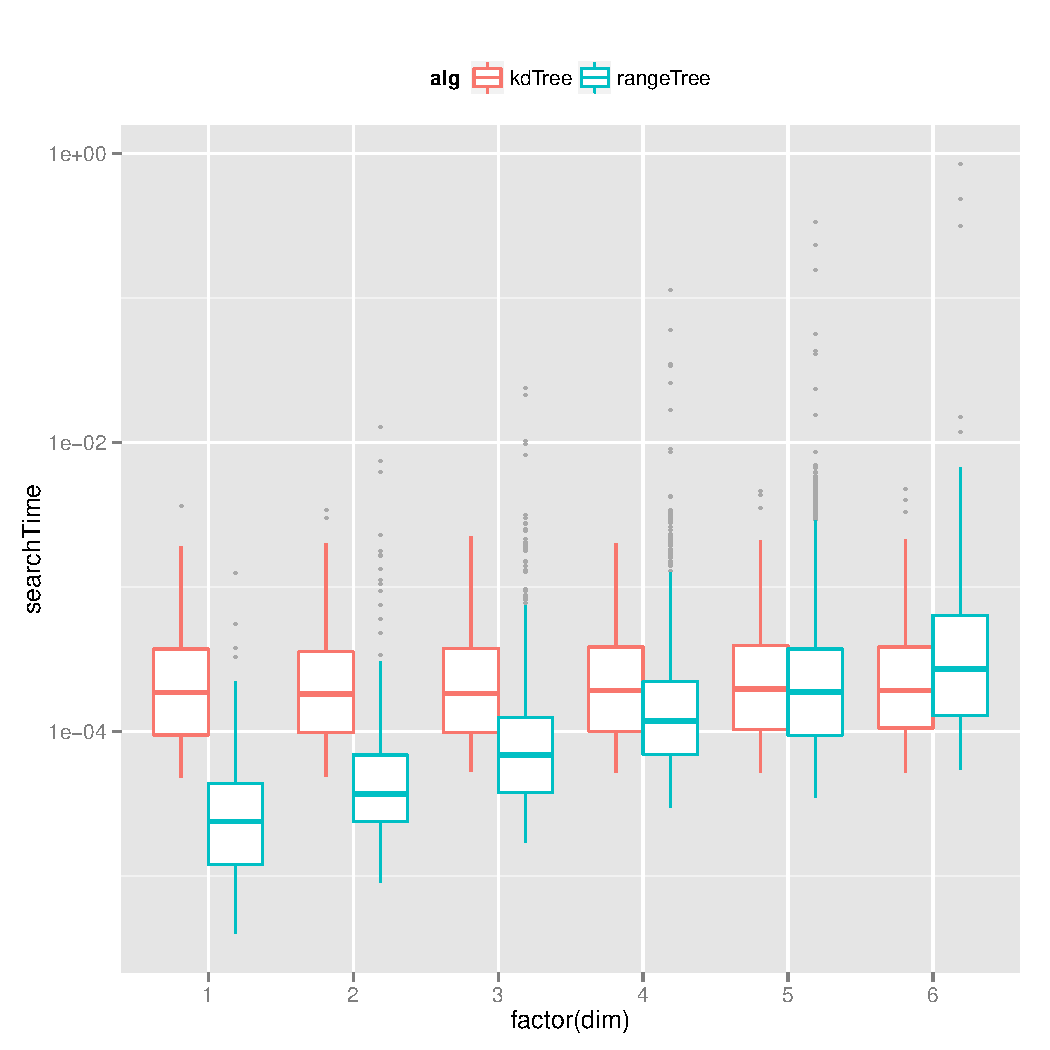
\includegraphics[width=\textwidth]{../src/R/plots/boxplot.pdf}
    \caption{}
\end{figure}
Figure 1 is a box-plot of each algorithms search time for each dimension on all 
input sizes. It is important to notice the logarithmic scale of the $y$ axis as 
some outliers are very fare form the norm. This is especially noticeable for the 
range tree. Since the range tree has enormous memory usage this might be due to 
cache misses.

Also note that the range tree is faster than the kd-tree for dimensions below 6.
\begin{figure}[H]
    \centering
    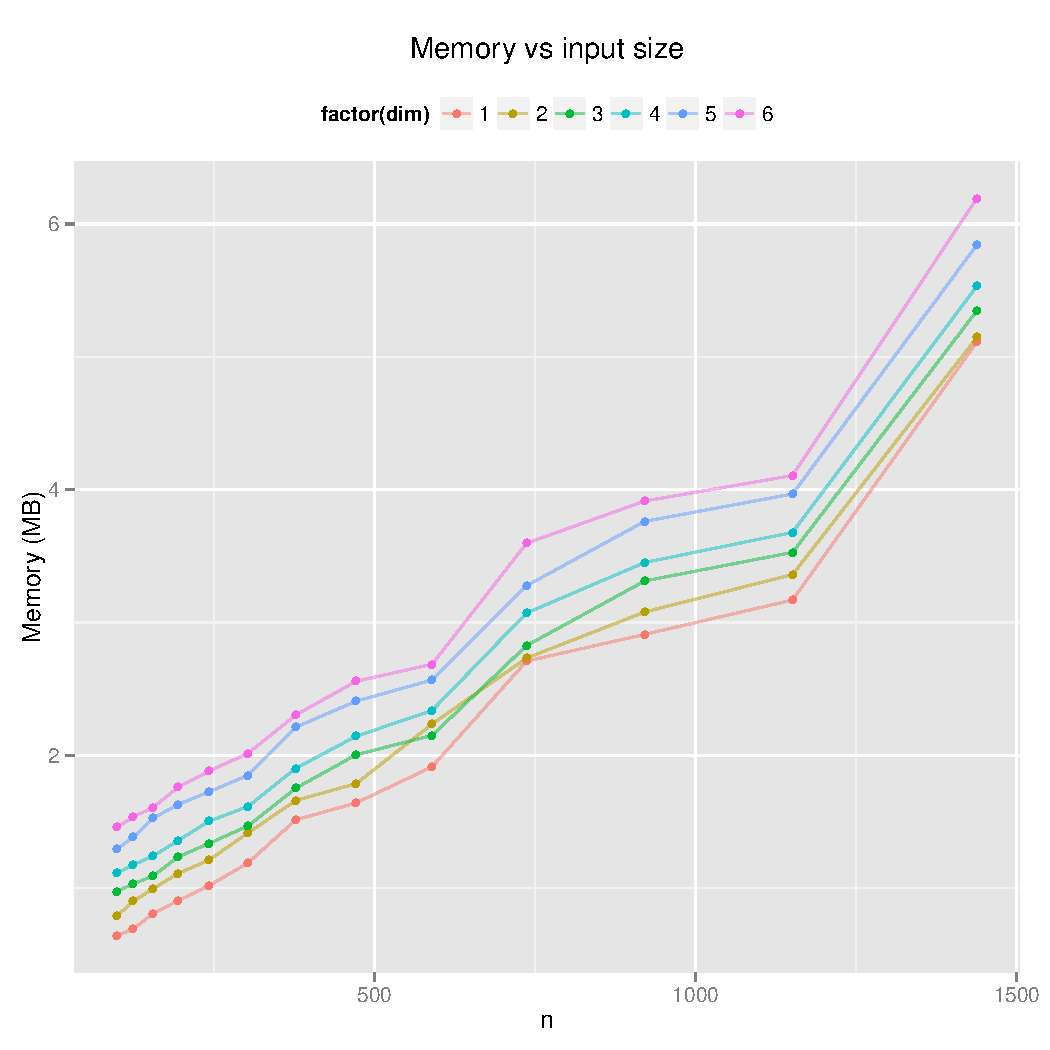
\includegraphics[width=\textwidth]{../src/R/plots/kdmem.pdf}
    \caption{}
\end{figure}
Figure 2: The memory usage of the kd-tree, notice the y-range from 2 trough 6 Mb, for elements 100 to roughly 1500. Also the size doesn't really grow
when the number of dimensions increases, except for the obvious increase in number of floats used to describe each point.
\begin{figure}[H]
    \centering
    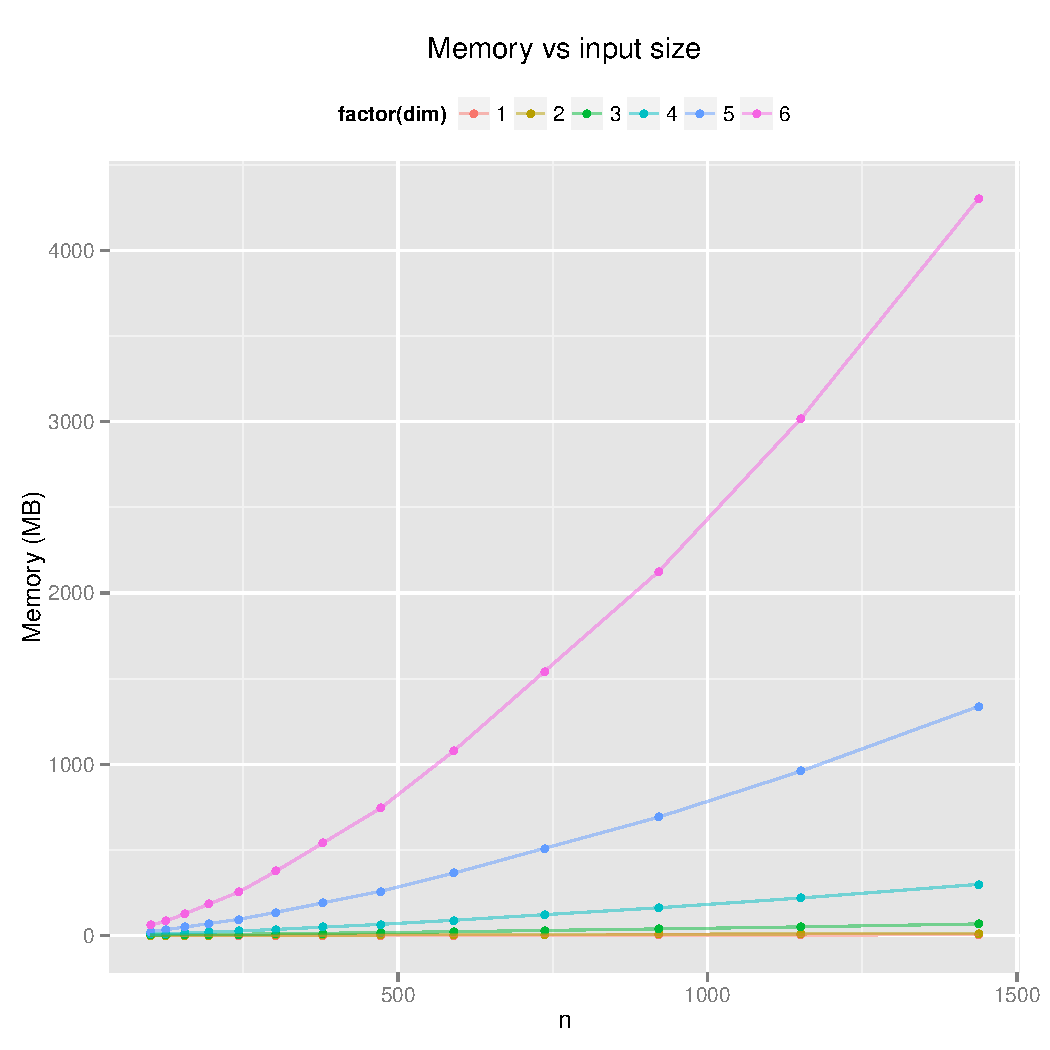
\includegraphics[width=\textwidth]{../src/R/plots/rtmem.pdf}
    \caption{}
\end{figure}
Figure 3: The memory usage of the range tree, notice the y-range from 2 trough 4300 Mb, for elements 100 to roughly 1500.
Now for each dimension, the memory used increases monstrous when the number of dimensions increases. Which makes it unsuitable for real life applications.
\newpage
\section{Conclusion}
\end{document}